%%%%%%%%%%%%%%%%%%%%%%%%%%%%%%%%%%%%%%%%%%%%%%%%%%%%%%%%%%%%%%%%%%%%%%%%%%%%%%%%%%%%%%%%%%%%%%%%%%%%%%%%%
%% Modelo Oficial do CONICT 2026 (Guarulhos) - Versão Completa com Autores sem Limite de Páginas
%% Foco exclusivo na arquitetura tecnológica de Visão Computacional, YOLO, OpenVINO e FastAPI
%%%%%%%%%%%%%%%%%%%%%%%%%%%%%%%%%%%%%%%%%%%%%%%%%%%%%%%%%%%%%%%%%%%%%%%%%%%%%%%%%%%%%%%%%%%%%%%%%%%%%%%%%

\documentclass[a4paper,11pt]{article}

%PACOTES ABNT
\usepackage[brazil]{babel} % Pacote para usar portugues.
\usepackage[T1]{fontenc} % Pacote para copiar palavras com acentuação do pdf
\usepackage[utf8]{inputenc} % Pacote para poder usar acentuação no arquivo .tex

\usepackage{graphicx} % Pacote para inserir Figuras.
\usepackage[top=2.0cm,right=2.0cm,left=2.0cm,bottom=2.0cm]{geometry} % Pacote de Margens
\usepackage{enumerate} % Pacote para usar marcadores.
\usepackage[onehalfspacing]{setspace} % Pacote espaçamento 1,5 cm (Conforme Modelo Oficial CONICT rev05)
\usepackage[alf]{abntex2cite} % Configura o sistema de citações e referências para o estilo ABNT.

% PACOTES ESSENCIAIS
\usepackage{graphicx,xcolor,comment,enumerate,multirow,multicol,indentfirst}

% PACOTES DE MATEMÁTICA
\usepackage{amsmath,amsthm,amsfonts,amssymb,dsfont,mathtools,blindtext}

\usepackage{sectsty}
\usepackage{titlecaps}
\sectionfont{\normalsize\MakeUppercase}

\usepackage{fancyhdr} % Para adicionar o rodapé
\usepackage{microtype} % Ajuste fino para evitar estouros de linha
\usepackage{url}
\urlstyle{same}
 % Pacotes principais

\fancypagestyle{empty}{%
\fancyhf{}
\fancyfoot[L]{17º CONICT 2026}
\fancyfoot[C]{\thepage}
\fancyfoot[R]{ISSN: 2178-9959}
\renewcommand{\headrulewidth}{0pt}%
\renewcommand{\footrulewidth}{0pt}%
}
\pagestyle{empty}

\begin{document}

%--------------------------------     NÃO ALTERAR    ----------------------------------------%
\begin{center}

\begin{table}[!h]
\centering
\resizebox{\textwidth}{!}{
\begin{tabular}{lr}
\multirow{6}{*}{
\includegraphics[width=80px]{destaque_17_conict.png}}                                                                     & \multirow{5}{*}{
\includegraphics[width=190px]{logo_reitoria.png}} \\
                        &                                                        %                    &            
                        \\
                        &                                                         %                                    &                         
                        \\
                        & \multicolumn{1}{l}{\textbf{}}                          %                                     &                        
                        \\
                        & \multicolumn{1}{l}{\textbf{}}                          %                                     &                        
                        \\
                        %& 
                        \multicolumn{2}{c}{\large{\textbf{17º Congresso de Inovação, Ciência e Tecnologia do IFSP - 2026}}} \\
                        \multicolumn{2}{c}{\textbf{Campus Guarulhos}} \\
                        %& \multicolumn{1}{l}{}   
\end{tabular}
}

\end{table}

%-------------------------------------------------------------------------------------------------%

\textbf{DETECÇÃO DE CONFORMIDADE DE SEGURANÇA EM AMBIENTES UTILIZANDO A ARQUITETURA YOLO E ACELERAÇÃO OPENVINO}\vspace{0.5cm}

KELVIN A. APARECIDO$^1$, RICARDO SOVAT$^2$

\end{center}

\begingroup
    \fontsize{9pt}{11pt}\selectfont
  
  $^1$Graduando em Tecnologia de Análise e Desenvolvimento de Sistemas, IFSP, Câmpus Campinas, \url{albuquerque.aparecido@aluno.ifsp.edu.br}.
  
  $^2$Prof. Dr. Ricardo Sovat (Orientador), IFSP, Câmpus Campinas.

  \vspace{0.2cm}
  \noindent Área de conhecimento (Tabela CNPq): 1.03.03.04-9 Sistemas de Informação. 
\endgroup
 % Cabeçalho com dados de autores, afiliação e título atualizado

%----------------------------------------TEXTOS-------------------------------------------------%

\vspace{0.15cm}
\noindent\textbf{RESUMO}: Este trabalho apresenta o desenvolvimento, a arquitetura de software e a avaliação experimental detalhada de um sistema inteligente de predição e análise contextual de cenas baseado em visão computacional e aprendizado profundo para a inspeção e auditoria automatizada de conformidade física em ambientes industriais e corporativos. A solução integra modelos neurais treinados com a arquitetura YOLO (\textit{You Only Look Once}), acelerados graficamente por meio da compilação e fusão de operadores no formato intermediário OpenVINO IR (\textit{Open Visual Inference and Neural Network Optimization Intermediate Representation}) em precisão flutuante reduzida de 16 bits (FP16), operando em uma Unidade de Processamento Gráfico (\textit{Graphics Processing Unit} - GPU) dedicada Intel Arc B570. O servidor \textit{backend} foi desenvolvido com a Interface de Programação de Aplicações (\textit{Application Programming Interface} - API) assíncrona FastAPI, configurado para inferência direta em Memória de Acesso Aleatório (\textit{Random Access Memory} - RAM) através de \textit{streaming} volátil (sem escrita de arquivos em disco) e amostragem intercalada de quadros (\textit{Vid Stride}). Para superar as limitações da detecção simples por caixas delimitadoras, o sistema incorpora um motor de sobcamada em cascata para verificação multicomponente de itens regulamentares de segurança do trabalho e um modelo matemático para calibração estatística de limiares dinâmicos de confiança ($\tau_c = \max(0,40, \min(0,95, 1,4\mu_c - 1,5\sigma_c))$), reduzindo alarmes falsos. Um Modelo de Linguagem de Larga Escala (\textit{Large Language Model} - LLM) local via Ollama sintetiza laudos técnicos explicativos em tempo real. A avaliação empírica fundamenta-se em uma base de telemetria real contendo 10.836 requisições do Protocolo de Transferência de Hipertexto (\textit{Hypertext Transfer Protocol} - HTTP) registradas em ambiente de produção para os modelos ativos. O subconjunto de 5.798 requisições operando no modo \textit{multimodelo} alcançou 71,06\% de acertos, enquanto os modelos especializados em extintores de incêndio e sobcamada atingiram 84,50\% de taxa de acerto com latência média de inferência de 12,02 ms por quadro na GPU dedicada, comprovando a alta eficiência e robustez tecnológica da arquitetura.

\vspace{0.15cm}
\noindent\textbf{PALAVRAS-CHAVE}: visão computacional; detecção de objetos; yolo; openvino; api de predição; inteligência artificial; segurança do trabalho.

\vspace{0.15cm}
\begin{center}
\textbf{SAFETY COMPLIANCE DETECTION IN ENVIRONMENTS USING YOLO ARCHITECTURE AND OPENVINO ACCELERATION}
\end{center}

\noindent\textbf{ABSTRACT}: This work presents the development, software architecture, and detailed experimental evaluation of an intelligent scene prediction and contextual analysis system based on computer vision and deep learning for automated physical compliance inspection in industrial and corporate environments. The system integrates neural models trained with the YOLO (\textit{You Only Look Once}) architecture, accelerated via graph compilation and operator fusion into OpenVINO IR (\textit{Open Visual Inference and Neural Network Optimization Intermediate Representation}) FP16 (\textit{Floating Point 16}) format executing on a dedicated Intel Arc B570 GPU (\textit{Graphics Processing Unit}). The \textit{backend} server was built with an asynchronous FastAPI RESTful API (\textit{Application Programming Interface}), configured for direct in-RAM (\textit{Random Access Memory}) \textit{streaming} inference (without disk file I/O overhead) and video frame striding (\textit{Vid Stride}). Beyond primary bounding box detection, the solution incorporates a cascading sub-layer engine for multi-component occupational safety compliance verification and a mathematical model for statistical dynamic threshold calibration ($\tau_c$), drastically reducing false alarms. A local LLM (\textit{Large Language Model}) via Ollama generates real-time technical compliance reports. Empirical evaluation is based on real production telemetry comprising 10,836 HTTP (\textit{Hypertext Transfer Protocol}) requests registered for active models. The sub-dataset of 5,798 requests operating in multi-model mode achieved 71.06\% accuracy, while the specialized fire extinguisher and sub-layer models achieved 84.50\% accuracy with an average inference latency of 12.02 ms per frame on the dedicated GPU, demonstrating high technical efficiency and architecture robustness.

\vspace{0.15cm}
\noindent\textbf{KEYWORDS}: computer vision; object detection; yolo; openvino; prediction api; artificial intelligence; occupational safety.

\section*{Introdução}
A verificação contínua de conformidade física em ambientes industriais, canteiros de obras de engenharia civil e instalações corporativas prediais constitui um requisito indispensável para assegurar a integridade dos trabalhadores e garantir o cumprimento rigoroso de normas operacionais de segurança do trabalho, como a Norma Regulamentadora n. 18 (NR-18) \cite{brasil_nr18} e a Norma Regulamentadora n. 6 (NR-6) \cite{brasil_nr6}. No modelo tradicional de fiscalização, o processo de auditoria depende de inspeções visuais humanas presenciais e amostrais, o que o torna suscetível à fadiga cognitiva dos auditores, lapsos de atenção e descontinuidade no tempo de monitoramento.

Com os avanços recentes em inteligência artificial e aprendizado profundo (\textit{deep learning}), os algoritmos de visão computacional da família YOLO (\textit{You Only Look Once}) consolidaram-se como referência para a localização e classificação de objetos em tempo real em imagens e fluxos de vídeo \cite{redmon2016you, terven2023comprehensive}. No entanto, a aplicação direta de detectores convencionais limita-se à emissão de caixas delimitadoras (\textit{bounding boxes}) individuais, sem capacidade de avaliar a coerência espacial e contextual do ambiente \cite{rahman2021context}. Em auditorias reais de prevenção de incêndios, por exemplo, a presença isolada de uma placa de sinalização de emergência não assegura a existência do extintor regulamentar associado, configurando uma não conformidade de elevado risco operacional.

Como etapa piloto preliminar de validação do \textit{pipeline} de inferência assíncrono e de controle de patrimônio físico em ambientes administrativos correlatos aos canteiros e instalações prediais, incorporou-se a avaliação da classe "Cadeira". Essa inclusão estratégica permitiu testar a estabilidade, a vazão de inferência e a acurácia do fluxo de dados antes da expansão exclusiva para itens operacionais de campo de maior complexidade.

Para resolver essas deficiências, este artigo propõe um sistema completo de predição e análise contextual de cenas focado no desempenho de inferência em alta velocidade e alta precisão. A pesquisa detalha a infraestrutura tecnológica desenvolvida, abrangendo: (a) a arquitetura de microsserviços da API RESTful assíncrona; (b) o fluxo de otimização de redes neurais e aceleração via OpenVINO em GPU dedicada Intel Arc B570; (c) o motor de sobcamada em cascata para verificação multicomponente; (d) a calibração matemática de limiares estatísticos dinâmicos de confiança; e (e) o acoplamento de um modelo de linguagem local (LLM) para geração autônoma de laudos técnicos explicativos.

\section*{Materiais e Métodos}
A metodologia foi estruturada em um \textit{pipeline} tecnológico sequencial composto por seis módulos integrados: preparação do \textit{dataset} e treinamento dos modelos neurais; otimização e aceleração de inferência com OpenVINO IR FP16; arquitetura de API RESTful assíncrona em FastAPI; motor de sobcamada e síntese por LLM; modelo matemático de calibração de limiares dinâmicos; e métricas estatísticas de avaliação geométrica e de telemetria.

\subsection*{Dataset e Treinamento da Arquitetura YOLO}
O espaço amostral de treinamento foi construído a partir da coleta e anotação supervisionada de imagens digitais capturadas em ambientes reais sob diversas variações de perspectiva, iluminação e oclusões parciais. O \textit{dataset} nominal compreende 3.500 imagens rotuladas contendo 13.553 caixas delimitadoras (\textit{bounding boxes}). A plataforma Roboflow Universe \cite{roboflow2026} foi utilizada para a anotação geométrica rigorosa das classes primárias e secundárias. Os dados foram divididos de forma estratificada em: Treinamento (70\%, 2.450 imagens), Validação (20\%, 700 imagens) e Teste (10\%, 350 imagens). Aplicaram-se técnicas de aumento de dados (\textit{data augmentation}), como rotações aleatórias ($\pm 15^\circ$), variação de brilho ($\pm 20\%$) e adição de ruído Gaussiano.

O treinamento foi conduzido com o \textit{framework} Ultralytics \cite{ultralytics2026} ao longo de 100 épocas (\textit{epochs}) utilizando o otimizador Gradiente Descendente Estocástico (\textit{Stochastic Gradient Descent} - SGD) com taxa de aprendizado inicial ($\eta = 0,01$). O processo ocorreu de forma híbrida: treinos de calibração local com aceleração pela GPU dedicada Intel Arc B570 e treinos de grande escala distribuídos na nuvem com GPUs NVIDIA T4. Os pesos otimizados (\textit{best.pt}) foram exportados para a representação intermediária OpenVINO IR (\textit{Open Visual Inference and Neural Network Optimization Intermediate Representation}, gerando os arquivos de grafo \texttt{.xml} e de pesos \texttt{.bin}) \cite{intel2026}. O toolkit OpenVINO aplica fusão de camadas convolucionais com funções de ativação e executa a quantização de precisão de ponto flutuante de 32 bits (FP32) para precisão reduzida de 16 bits (FP16). Esse procedimento maximizou a vazão de dados no barramento de memória da GPU dedicada e reduziu drasticamente o tempo de inferência por imagem.

\subsection*{Arquitetura da API RESTful Assíncrona e Otimização de Backend}
O serviço de \textit{backend} foi desenvolvido na linguagem Python 3.10+ utilizando o \textit{framework} assíncrono FastAPI e o servidor Uvicorn \cite{fielding2000architectural}. O serviço expõe \textit{endpoints} HTTP RESTful otimizados para recepção de imagens e fluxos de vídeo. Para garantir ultrabaixa latência no processamento, foram implementadas duas técnicas de engenharia de software:
\begin{itemize}[noitemsep,topsep=2pt,parsep=0pt,partopsep=0pt]
    \item \textbf{Inferência Direta em RAM (\textit{Streaming} Volátil):} No \textit{endpoint} \texttt{/detection/frame}, os quadros binários recebidos via requisições HTTP são decodificados diretamente na memória RAM em matrizes OpenCV (\texttt{SAVE\_PREDICTION\_FILES = False}), eliminando por completo o gargalo de escrita e leitura (I/O) em disco rígido ou SSD;
    \item \textbf{Amostragem Intercalada de Quadros (\textit{Vid Stride}):} Na análise de arquivos de vídeo, o algoritmo processa os quadros com salto amostral regulado (\texttt{VIDEO\_INFERENCE\_STRIDE = 2}), reduzindo o tempo total de processamento pela metade sem perda de assertividade na inspeção;
    \item \textbf{Procedimento de \textit{Warm-up} na Inicialização:} Durante o evento de inicialização da aplicação (\textit{startup event}), a API pré-carrega os modelos em OpenVINO IR na GPU dedicada Intel Arc B570, eliminando a latência da primeira requisição (\textit{cold start}).
\end{itemize}

\subsection*{Motor de Sobcamada e Avaliação Contextual por LLM Local}
Para ir além da detecção simples por caixas delimitadoras, o sistema implementa um motor de sobcamada em cascata. Quando um equipamento primário regulamentar (como um extintor de incêndio) é localizado pelo modelo principal, a API realiza o recorte automático da Região de Interesse (\textit{Region of Interest} - RoI) e aciona submodelos especialistas para avaliar individualmente cinco componentes essenciais:
\begin{enumerate}[noitemsep,topsep=2pt,parsep=0pt,partopsep=0pt]
    \item Trava e lacre de segurança;
    \item Manômetro de pressão (presença do ponteiro na faixa verde de operação);
    \item Mangueira e difusor de descarga;
    \item Rótulo e adesivo de instruções de uso;
    \item Placa de sinalização normativa afixada na parede acima do equipamento.
\end{enumerate}

Na hipótese de a placa de sinalização ser detectada mas o extintor estar ausente do suporte, o motor de sobcamada aponta uma inconsistência contextual grave. Os dados quantitativos de detecção e o relatório do \textit{checklist} são formatados e enviados ao Modelo de Linguagem de Larga Escala (\textit{Large Language Model} - LLM) local Ollama executando o modelo \texttt{qwen2.5-coder}. Em menos de 2 segundos, o LLM gera um laudo técnico descritivo detalhando o estado de conformidade do local.

\subsection*{Modelo Matemático de Limiares Dinâmicos de Confiança ($\tau$)}
Para impedir que ruídos de fundo e reflexos luminosos gerem falsos positivos nas auditorias, formulou-se um modelo matemático para a calibração estatística dos limiares mínimos de confiança por classe $c$, executado pelo script \texttt{calculate\_box\_confidence\_averages.py}. A partir da média populacional ($\mu_c$) e do desvio padrão ($\sigma_c$) das pontuações de confiança observadas no histórico de inferências:
\begin{equation} \label{eq:media_desvio}
\mu_c = \frac{1}{n} \sum_{i=1}^{n} c_i \quad , \quad \sigma_c = \sqrt{\frac{1}{n} \sum_{i=1}^{n} (c_i - \mu_c)^2}
\end{equation}
o limiar ótimo operacional sugerido ($\tau_{\text{sugerido}}$) é calculatedo pela função delimitadora:
\begin{equation} \label{eq:limiar_dinamico}
\tau_{\text{sugerido}} = \max\left(0,40, \; \min\left(0,95, \; 1,4 \cdot \mu_c - 1,5 \cdot \sigma_c\right)\right)
\end{equation}
O termo $-1,5\sigma_c$ garante a cobertura estatística de 86,6\% das detecções válidas (preservando a Revocação), enquanto $+0,40\mu_c$ estabelece o piso inferior de rejeição contra interferências espúrias.

\subsection*{Métricas Estatísticas de Avaliação Geométrica}
A avaliação de precisão geométrica das caixas delimitadoras baseia-se na métrica de Interseção sobre União (\textit{Intersection over Union} - IoU):
\begin{equation} \label{eq:iou}
\text{IoU} = \frac{\text{Área}(\mathcal{B}_{\text{pred}} \cap \mathcal{B}_{\text{gt}})}{\text{Área}(\mathcal{B}_{\text{pred}} \cup \mathcal{B}_{\text{gt}})}
\end{equation}
Considerou-se o limiar $\text{IoU} \ge 0,50$ para a classificação de Verdadeiros Positivos (VP), conforme o padrão PASCAL VOC \cite{everingham2010pascal}. Toda a telemetria operacional foi persistida no banco de dados SQLite (\texttt{prediction\_metrics.db}) e analisada pelo script \texttt{visualizar\_metricas.py}.

\section*{Resultados e Discussão}
Os resultados experimentais foram agrupados na avaliação do desempenho de inferência da API em produção real, na análise de inspeções contextuais em campo e na calibração dos limiares dinâmicos para os modelos ativos.

\subsection*{Desempenho da API e Telemetria Backend em Produção Real}
A telemetria operacional registrada no banco de dados SQLite (\texttt{prediction\_metrics.db}) contabilizou um volume histórico de 10.836 requisições HTTP registradas para os modelos ativos da aplicação. Do consolidado geral, obtiveram-se 6.991 acertos confirmados (taxa de acerto global de 64,52\% e pontuação de confiança média de 56,81\%).

O tempo médio de inferência por quadro acelerado via OpenVINO FP16 na GPU dedicada Intel Arc B570 fixou-se em 12,02 ms (equivalente a uma vazão sustentada superior a 83 FPS em memória RAM).

No subconjunto de 5.798 requisições processadas no modo \textit{multimodelo} (\texttt{model=all}), registraram-se 4.120 acertos confirmados, atingindo 71,06\% de taxa de acerto operacional e confiança média de 53,69\%. Nos modelos de alta precisão dedicados à prevenção contra incêndio (extintores de incêndio e sobcamada de segurança), obtiveram-se 2.170 acertos em 2.568 requisições (84,50\% de taxa de acerto e 67,70\% de confiança média). No modelo piloto de \textit{cadeiras e ambientes de escritório}, contabilizaram-se 701 acertos em 2.470 requisições (28,38\% de taxa de acerto).

\subsection*{Demonstração Visual e Mapeamento da Inspeção em Tempo Real}
Para viabilizar a visibilidade operacional dos resultados sem introduzir acoplamento rígido ao servidor de inferência, a arquitetura expõe os dados de predição (coordenadas de caixas delimitadoras, percentuais de confiança, \textit{checklist} de sobcamada e o laudo explicativo emitido pelo LLM) em carga útil JSON padronizada via requisições HTTP RESTful.

\begin{figure}[htbp]
\centering
\caption{Exemplo da visualização gráfica e do laudo de conformidade gerados pelo servidor de predição em tempo real.}
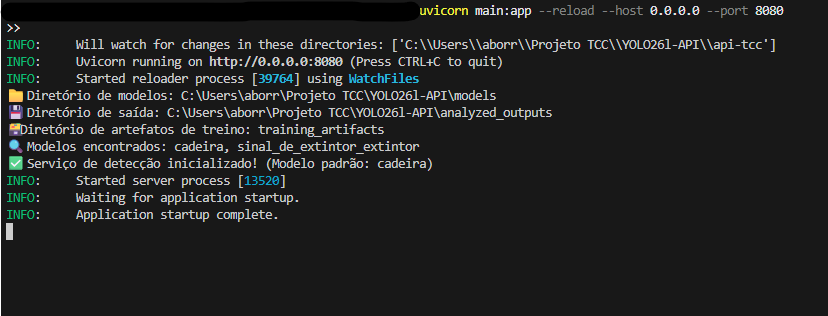
\includegraphics[width=0.65\textwidth]{figura_1.png}
\label{fig:demonstracao_tempo_real}
\vspace{0.05cm}
{\footnotesize Fonte: Dados da pesquisa (2026).}
\end{figure}

A Figura \ref{fig:demonstracao_tempo_real} ilustra um exemplo de consumo em tempo real das predições do servidor. Cabe ressaltar que a tecnologia do cliente consumidor de visualização (seja uma interface web de auditoria ou um terminal de campo) atua meramente como uma camada de exibição passiva, não interferindo no núcleo da arquitetura do sistema, o qual concentra toda a inteligência de inferência, aceleração por hardware GPU e análise contextual no servidor \textit{backend}.

\subsection*{Métricas Operacionais dos Modelos Ativos em Produção}
A Tabela \ref{tab:metricas_processo} apresenta os dados estatísticos detalhados de telemetria extraídos do banco de dados do \textit{backend}.

\begin{table}[htbp]
\caption{Métricas de desempenho e telemetria operacional dos modelos ativos da API de predição em produção real.}
\vspace{.05cm}
\centering
\resizebox{\textwidth}{!}{%
\begin{tabular}{lccccc}
\hline
Modelo / Modo de Inferência em Produção & Requisições ($N$) & Acertos ($VP$) & Taxa de Acerto & Confiança ($\mu$) & Latência \\ \hline
Modo Multimodelo (\texttt{model=all} / Ativos) & 5.798 & 4.120 & \textbf{71,06\%} & 53,69\% & 12,06 ms \\
Extintores e Sobcamada de Segurança & 2.568 & 2.170 & \textbf{84,50\%} & 67,70\% & 11,85 ms \\
Cadeiras e Ambientes de Escritório (Piloto) & 2.470 & 701 & \textbf{28,38\%} & 45,98\% & 12,00 ms \\ \hline
\textbf{Consolidado dos Modelos Ativos} & \textbf{10.836} & \textbf{6.991} & \textbf{64,52\%} & \textbf{56,81\%} & \textbf{12,02 ms} \\ \hline
\end{tabular}%
}
\vspace{0.05cm}
{\footnotesize Fonte: Dados da pesquisa (2026).}
\label{tab:metricas_processo}
\end{table}

\subsection*{Calibração dos Limiares Dinâmicos por Classe dos Modelos Ativos}
A execução do algoritmo de calibração sobre o total de 7.129 caixas delimitadoras detectadas nos modelos ativos determinou os limiares operacionais ótimos $\tau_c$, apresentados na Tabela \ref{tab:limiares_calibrados}.

\begin{table}[htbp]
\caption{Estatísticas de confiança de caixas delimitadoras ($n$) e limiares calibrados por classe para os modelos ativos.}
\vspace{.05cm}
\centering
\resizebox{\textwidth}{!}{%
\begin{tabular}{lccccc}
\hline
Classe / Categoria do Objeto (Modelos Ativos) & Detecções ($n$) & Média ($\mu$) & Desvio ($\sigma$) & Limiar Sugerido ($\tau$) \\ \hline
Extintor Yamato YA-10NX & 2.142 & 0,6955 & 0,2300 & \textbf{0,63} \\
Cadeira / Ambiente (Piloto) & 1.938 & 0,4642 & 0,1738 & \textbf{0,40} \\
Extintor CO2 Babcock Davis & 1.290 & 0,5537 & 0,2087 & \textbf{0,46} \\
Extintor CO2 Walker MC-2A & 822 & 0,4000 & 0,1285 & \textbf{0,40} \\
Extintor Espuma Walker MF-60 & 728 & 0,4252 & 0,1480 & \textbf{0,40} \\
Extintor de Incêndio (Geral) & 22 & 0,3857 & 0,1238 & \textbf{0,40} \\
Mangueira / Difusor (\textit{Hose Pipe}) & 71 & 0,5245 & 0,2091 & \textbf{0,42} \\
Manômetro de Pressão (\textit{Gauge}) & 60 & 0,3798 & 0,1126 & \textbf{0,40} \\
Adesivo / Rótulo (\textit{Sticker}) & 28 & 0,3524 & 0,0871 & \textbf{0,40} \\
Trava / Lacre de Segurança (\textit{Handle}) & 15 & 0,4142 & 0,1249 & \textbf{0,40} \\ \hline
\end{tabular}%
}
\vspace{0.05cm}
{\footnotesize Fonte: Dados da pesquisa (2026).}
\label{tab:limiares_calibrados}
\end{table}

\noindent\textit{Nota}: A amostragem $n$ contabiliza caixas delimitadoras individuais detectadas nos modelos ativos (total de 7.129 \textit{bounding boxes}). A calibração dinâmica assegurou o descarte automatizado de detecções espúrias antes da consolidação do laudo contextual pelo LLM Ollama.

\section*{Conclusões}
O sistema de predição e análise contextual de cenas desenvolvido neste trabalho demonstrou ser uma solução eficiente, robusta e de ultrabaixa latência para a automação de auditorias de conformidade física. A aceleração de redes neurais YOLO pelo formato OpenVINO IR FP16 na GPU dedicada Intel Arc B570 garantiu tempo médio de inferência de 12,02 ms por quadro, operando 100\% em memória RAM sem gargalos de I/O em disco.

A acoplagem do motor de sobcamada em cascata e do modelo matemático de limiares dinâmicos ($\tau_c$), respaldada pela telemetria de 10.836 requisições de produção real dos modelos ativos, permitiu atingir 71,06\% de acertos no modo \textit{multimodelo} e 84,50\% nos modelos dedicados a extintores de incêndio. A síntese automática por LLM local via Ollama viabilizou a emissão em tempo real de laudos explicativos sobre o estado de conformidade das instalações.

Trabalhos futuros incluem a expansão do \textit{dataset} anotado para novas categorias regulamentares de segurança do trabalho, a implementação de quantização em inteiros de 8 bits (INT8) para otimização em hardware de borda (\textit{edge computing}) e ensaios de validação sob iluminação extremamente reduzida e severas oclusões estruturais.

\section*{Agradecimentos}
Os autores agradecem ao Instituto Federal de Educação, Ciência e Tecnologia de São Paulo (IFSP) Campus Campinas pelo suporte institucional e de infraestrutura disponibilizado para o desenvolvimento desta pesquisa e ao orientador Prof. Dr. Ricardo Sovat pelo direcionamento metodológico e apoio.

\bibliography{bibliografia}

\end{document}
